\section{Initial conditions}

We need to determine the initial shape of a bubble floating at a gas-liquid interface before it's film ruptures. This derivation is based on the work done in \cite{toba1959drop}.
We are considering the case where the fluid is stationary, i.e. $\bf{u} = \bf{0}$, meaning on the boundaries we only need to consider the Young-Laplace equation:
\begin{align}
    \Delta p=-\gamma \nabla \cdot \hat n
\end{align}

\begin{figure}[hb]
    \centering
    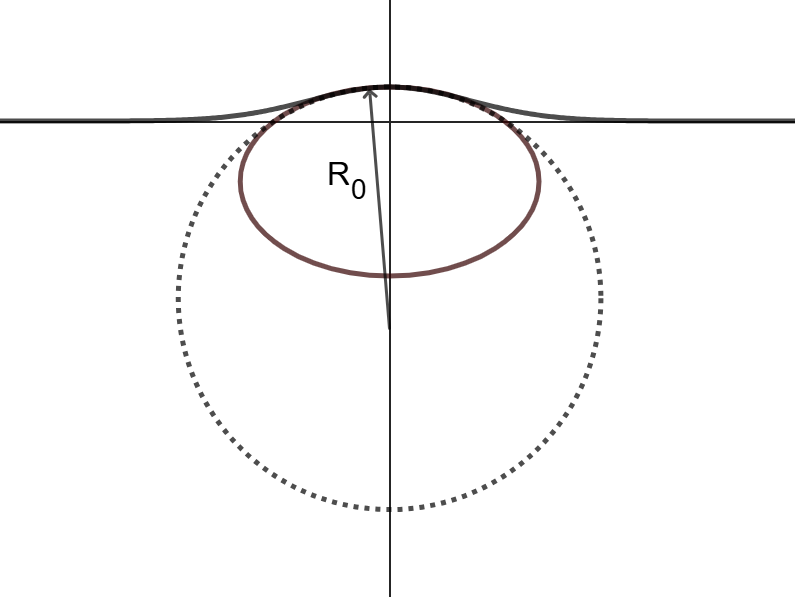
\includegraphics[width=0.55\linewidth]{WriteUp/images/bubble at surface.png}
    \caption{A bubble floating at a surface}
    \label{fig:1}
\end{figure}

We can divide the surface of a bubble into three regions: (A) the submerged portion of the interface, (B) the thin film over the top of the bubble separating the two gas regions, (C) the regions of the interface trailing away from the border of the thin film. We neglect the thickness of the film means we can ignore the weight of the film. Adding that the difference between the gas pressures inside and out of the bubble is uniform, the thin film can be treated as a spherical surface of radius $R_0$. The force balance equations at any point on these surfaces are,
\begin{align}
    (\rho-\rho')gz = \gamma(\frac{1}{R_1}+\frac{1}{R_2}-\frac{4}{R_0})
\end{align}
for region (A),
\begin{align}
    p=p_0 + \frac{4\gamma}{R_0}
\end{align}
for region (B),
\begin{align}
    (\rho-\rho')gz = \gamma(\frac{1}{R_1}+\frac{1}{R_2})
\end{align}
for region (C) where $\gamma$ represents surface tension of the liquid, $g$ is acceleration due to gravity, $\rho$ and $\rho'$ are the densities of the liquid and gas respectively, $p$ and $p_0$ are the gas pressure inside and outside the bubble respectively, $g$ is acceleration due to gravity and $z$ is the height above the still gas liquid interface in the far field. $R_1$ and $R_2$ are the principle radii of curvature of the surface at a point.

In order to calculate what $R_1$ and $R_2$ are we need to use some differential geometry. We assume the bubble can be described by a surfaces of revolution.
Let $\gamma$ be a curve that lies in the plane $(x,z)$ and let its equation have the equation $z=f(x)$. We then denote $\Phi$ as the surface defined by a rotation of $\gamma$ around the $z$-axis or axis of rotation. This surface can then be written in the form:
\begin{align}
    z=f(\sqrt{x^2+y^2})=f(r) && r=\sqrt{x^2+y^2}
\end{align}

Then using the formulas derived in \cite{toponogov2006differential} we get
\begin{align}
    E&=1+(\frac{x}{r}f')^2,&G&=1+(\frac{y}{r}f')^2, &F&=\frac{xy}{r^2}(f')^2, &EG-F^2=&1+(f')^2,
\end{align}
for the coefficients of the first fundamental form given by
\begin{align}
    I( \vec{ \boldsymbol\lambda}) = E(\lambda_1)^2 +2F\lambda_1 \lambda_2 + G(\lambda_2)^2
\end{align}
where $\lambda$ is some tangent vector. We can exploit the fact that since our surface is radially symmetric, we only need to find these geometric characteristics on some meridian of the surface, say y=0:
\begin{align}
    E&=1+(f')^2,& G&=1, &F&=0.
\end{align}
Again using the formulas in \cite{toponogov2006differential}, we obtain
\begin{align}
    L&=\frac{f''}{\sqrt{1+(f')^2}},&M&=0&  N&=\frac{f'}{x\sqrt{1+(f')^2}}
\end{align}
for the coefficients of the second fundamental form given by
\begin{align}
    II( \vec{ \boldsymbol\lambda},\vec{ \boldsymbol\mu}) = L\lambda_1 \mu_1 +M(\lambda_1\mu_2 + \lambda_2 \mu_1)  + N\lambda_2 \mu_2.
\end{align}
We then obtain the principle curvatures $\kappa_1$ and $\kappa_2$ satisfy:
\begin{align}
    (EG-F^2)\kappa^2 - (EN+GL -2MF)\kappa +LN-M^2 = 0.
\end{align}
Substituting in our coefficients for the first and second fundamental forms, solving for $K$ and noting radius of curvature is one over the curvature we obtain:
\begin{align}
    \frac{1}{K_1} =\kappa_1= \frac{L}{E}=\frac{f''}{(1+(f')^2)^{\frac{3}{2}}}, && \frac{1}{K_2} = \kappa_2 = \frac{N}{G} = \frac{f'}{x \sqrt{1+(f')^2}}
\end{align}
Notice that $K_1$ is exactly the curvature of the meridian curve $\gamma$
We now introduce the variable $\phi$ defined to be the angle at which the tangent to $\gamma$ makes with the x-axis. 
\begin{figure}[hb]
    \centering
    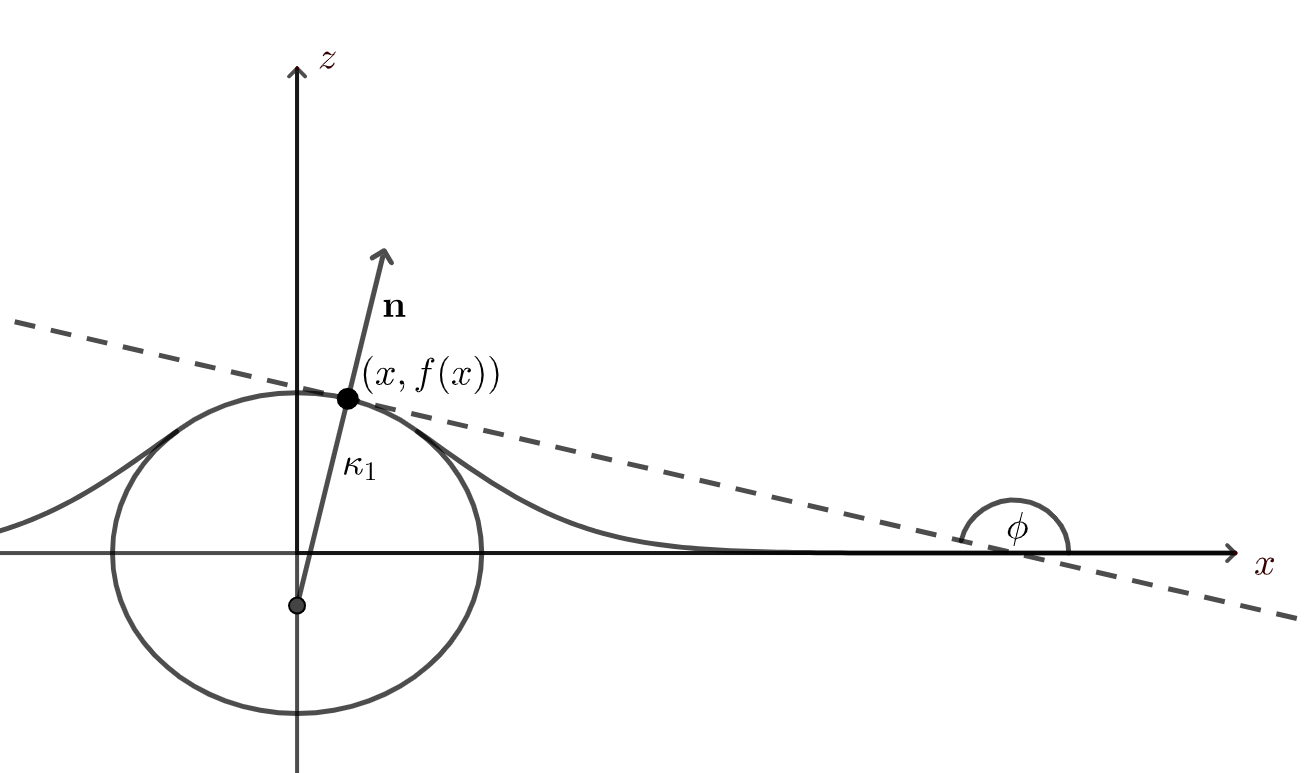
\includegraphics[width=0.55\linewidth]{WriteUp/images/tangent to bubble extra.png}
    \caption{A bubble floating at a surface}
    \label{fig:1}
\end{figure}
We can calculate $phi$ using simple trigonometry to be $\phi=\arctan(f'(x))$. We then consider:
\begin{align}
    f'(x)=\tan \phi &= \frac{\sin\phi}{\cos\phi} \\
    &=\sin\phi\sec\phi \\
    &=\sin\phi \sqrt{1+\tan^2\phi}\\
    \frac{f'(x)}{\sqrt{1+f'(x)^2}}&=\sin\phi\\
    \frac{d}{dx} \frac{f'(x)}{\sqrt{1+f'(x)^2}}&=\frac{d}{dx}\sin\phi \\
    \frac{f''(x)}{(1+f'(x)^2)}&=\frac{d(\sin\phi)}{dx} \\
    \frac{1}{K_1}&=\frac{d(\sin\phi)}{dx}
\end{align}
Allowing us to obtain $K_1$ in terms of $\phi$.
We can also write $K_2$ in terms of $\phi$ by considering the normal to the curve at a point $(x,f(x))$. An equation for this normal is given by
\begin{align}
    (\bar{x}-x) + f'(x)(\bar{z}-f(x))=0
\end{align}
where $(\bar{x},\bar{z})$ are the coordinates of points on the straight line. We can the find the intersection of this line with the $z$-axis, $(0,\frac{x+ff'}{f'})$.
Finding the distance between this point and $(x,f)$ gives
\begin{align}
    \sqrt{x^2+(\frac{x+ff'}{f'}-f)^2}=\frac{x\sqrt{1+(f')^2}}{|f'|}.
\end{align}